%%%%%%%%%%%%%%%%%%%%%%%%%% lecture-1
\begin{frame}
  \frametitle{lecture-3 主要内容}
  \framesubtitle{最简单的C语言程序设计---顺序程序设计}
  \tableofcontents[hideallsubsections]
\end{frame}

\section{数据的输入输出}

\begin{frame}{常用格式描述符与数据类型的对应关系}
\begin{tabular}{|c|c|c|}
	\hline 
	\textbf{格式符} & \textbf{对应的数据类型} &  \textbf{备注}\\ 
	\hline 
	\%d & int &  \\ 
	\hline  
	\%f & float &  \\
	\hline
	\%c & char & \\ 
	\hline   
	\%lf & double & \\ 
	\hline 
	\%.2f & float & 保留两位小数, 四舍五入。不适用于scanf()。 \\ 
	\hline 
	\%.2lf & double & 保留两位小数, 四舍五入。不适用于scanf()。 \\ 
	\hline
	\hline   
	\%x & int & 十六进制显示 \\ 
	\hline 
	\%ld & long int &  \\ 
	\hline 
\end{tabular}
\newline
\newline
\textcolor{blue}{详见p73, 表3.6}
\end{frame}

\begin{frame}[fragile]{输出语句printf(``原样输出, \%格式符'', 对应变量值);}
\begin{lstlisting}
#include<stdio.h>            // standard input/output编译预处理指令
int main()                   // 主函数
{                            // 函数开始标志
   int a=10,b;    // 定义变量a, b为整型数值, 定义变量时,可以指定变量的初值
   float f=10.2;  // 定义变量f为单精度浮点数
   double d; // 定义变量d为双精度浮点数
   char c;   // 定义变量c为单个英文字母
   f=10.2;
   d=20.356;
   c='A';
   printf("a=%d,b=%d,c=%c,f=%f,d=%.2lf\n",a,b,c,f,d); // %.2f, %.2lf保留两位小数
   return 0;                 // 函数执行完毕返回函数值0
}                            // 函数结束标志
\end{lstlisting}
\end{frame}

\begin{frame}[fragile]{输入语句scanf(``\%变量格式符'', \&变量名);}
\begin{lstlisting}
#include<stdio.h>            // standard input/output编译预处理指令
int main()                   // 主函数
{                            // 函数开始标志
   int a=10,b;    // 定义变量a, b为整型数值, 定义变量时,可以指定变量的初值
   float f=10.2;  // 定义变量f为单精度浮点数
   double d; // 定义变量d为双精度浮点数
   char c='A';   // 定义变量c为单个英文字母, 字符输入以后讲
   printf("请输入整数和浮点数, 空格隔开:\n"); // 提示语句[可选]
   scanf("%d%f",&a,&f);  // 尽量简单, 不要有其它字符和'\n'
   printf("请输入两个浮点数, 空格隔开:\n"); // 提示语句[可选]
   scanf("%f%lf",&f,&d);
   printf("a=%d,b=%d,c=%c,f=%f,d=%lf\n",a,b,c,f,d); // \n为换行符
   return 0;                 // 函数执行完毕返回函数值0
}                            // 函数结束标志
\end{lstlisting}
\end{frame}

\begin{frame}[fragile]{字符输出函数putchar}
\begin{lstlisting}
#include<stdio.h>
int main()
{
   char a = 'B',b = 'O',c = 'Y'; //定义3个字符变量并初始化
   putchar(a); //向显示器输出字符B
   putchar(b); //向显示器输出字符O
   putchar(c); //向显示器输出字符Y
   putchar ('\n'); //向显示器输出一个换行符
   return 0;
}
\end{lstlisting}
\end{frame}

\begin{frame}[fragile]{字符输入函数getchar, 遇到回车, 开始从缓冲区中接收字符。}
\begin{lstlisting}
#include<stdio.h>
int main()
{
   char a,b,c;  //定义字符变量a,b,c
   a = getchar();  //从键盘输入一个字符,送给字符变量a
   b = getchar();  //从键盘输入一个字符,送给字符变量b
   c = getchar();  //从键盘输入一个字符,送给字符变量c
   putchar(a);  //将变量a的值输出
   putchar(b);  //将变量b的值输出 
   putchar(c);  //将变量c的值输出
   printf("\na=%d,b=%d,c=%d,a=%c,b=%c,c=%c\n",a,b,c,a,b,c);
   return 0;
}
\end{lstlisting}
\end{frame}

\begin{frame}[fragile]{字符输入函数getchar, 遇到回车, 开始从缓冲区中接收字符。}
\begin{lstlisting}
char a,b,c;  //定义字符变量a,b,c
a = getchar();  //从键盘输入一个字符,送给字符变量a
b = getchar();  //从键盘输入一个字符,送给字符变量b
c = getchar();  //从键盘输入一个字符,送给字符变量c
putchar(a);  //将变量a的值输出
putchar(b);  //将变量b的值输出 
putchar(c);  //将变量c的值输出
printf("\na=%d,b=%d,c=%d,a=%c,b=%c,c=%c\n",a,b,c,a,b,c);
\end{lstlisting}
从键盘输入abc回车, 观察结果, 应该是正确的结果。
遇到回车, 开始从缓冲区中接收字符。
\end{frame}

\begin{frame}[fragile]{字符输入函数getchar, 遇到回车, 开始从缓冲区中接收字符。}
\begin{lstlisting}
a = getchar();  //从键盘输入一个字符,送给字符变量a
b = getchar();  //从键盘输入一个字符,送给字符变量\n
c = getchar();  //从键盘输入一个字符,送给字符变量b
putchar(a);  //将变量a的值输出a
putchar(b);  //将变量b的值输出\n 
putchar(c);  //将变量c的值输出b
printf("\na=%d,b=%d,c=%d,a=%c,b=%c,c=%c\n",a,b,c,a,b,c);
\end{lstlisting}
再运行一次程序, 输入a回车, 输入b回车, 输入c回车, 观察结果。\\
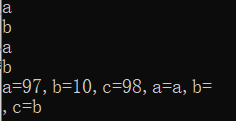
\includegraphics[scale=0.5]{abc}
\end{frame}

\section{数据类型}

\begin{frame}[fragile]{常量}
    \begin{lstlisting}
    #include<stdio.h> 
    #define PI 3.14  // 符号常量, 注意没有分号           
    int main()                   
    {                            
       int a = 123; // 整型常量
       float f = 12.2, f1=123E-1; // 实型常量
       char c1 = 'A', c2='\n'; // 字符常量
       char s[50] = "boy"; // 字符串常量      
       printf("回车换行\n");
       printf("单引号\',双引号\"转移字符前缀\,\n");  
       return 0;           
    }                            
    \end{lstlisting}
    \textcolor{blue}{转义字符, 见p40, 表3.1}
\end{frame}

\begin{frame}[fragile]{常变量}
\begin{lstlisting}
#include<stdio.h> 
#define PI 3.14  // 符号常量, 注意没有分号           
int main()                   
{                            
   int r = 123; // 整型变量
   const int a = 425; // 常变量
   r = 100; // 合法, 因为r是变量,可以随时更改它的值
   a = 100; // 不合法,因为a是常变量,不能更改
   printf("半径为%d的圆周长是%f\n",r,2*PI*r); 
   return 0;           
}                            
\end{lstlisting}
\end{frame}

\begin{frame}[fragile]{标识符}
标识符就是一个对象的名字。用于标识变量、符号常量、函数、数组、类型等。\\
\textcolor{blue}{以字母或下划线开始; 区分大小写; 不能使用关键字; 最好有含义。}
\begin{lstlisting}
#include<stdio.h>           
int main()                   
{                            
    int r = 123; // 合法整型变量名
    int 3a; // 不合法的变量名
    int brake; // 不合法的变量名, 因为break是关键字, 被系统使用。
    int Radius; // 变量名最好有含义
    int radius; // 与Radius是不同的变量,C语言是到小写敏感的语言
    return 0;           
}                            
\end{lstlisting}
\end{frame}

\begin{frame}{C语言关键字}
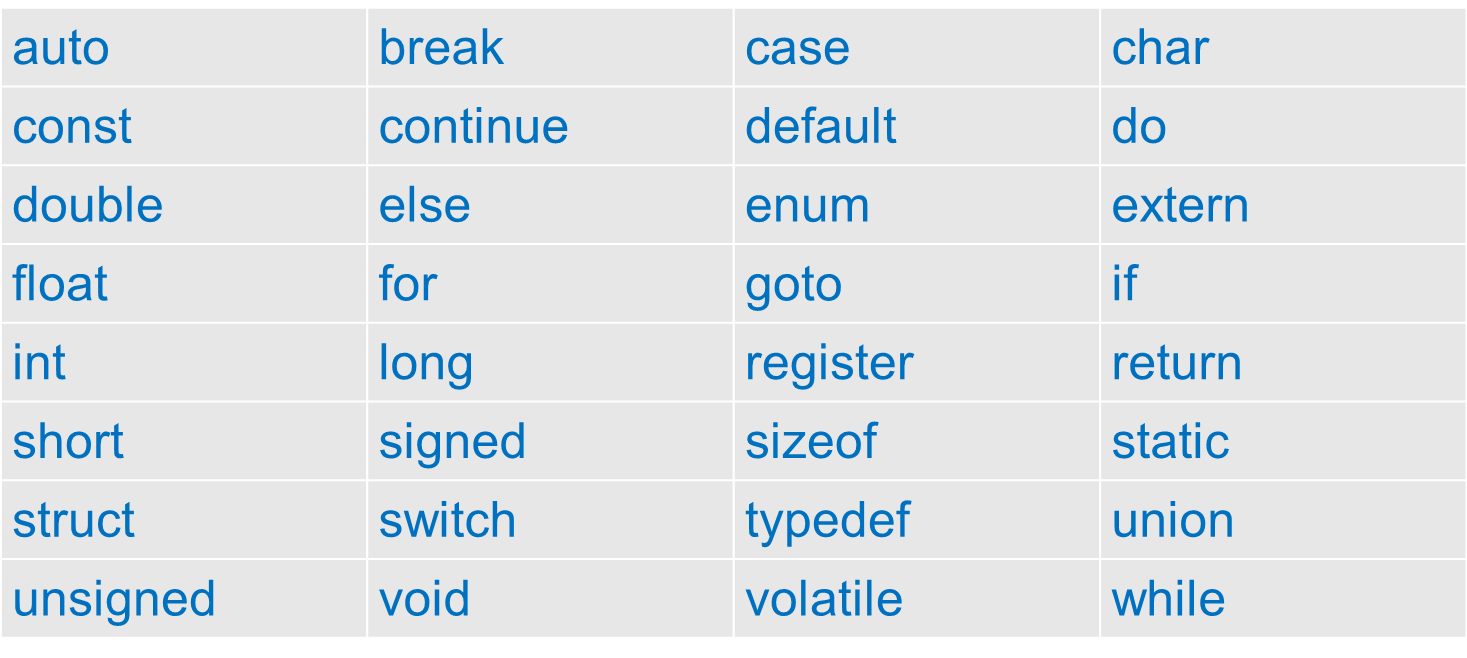
\includegraphics[scale=0.5]{key}
\end{frame}

\begin{frame}[fragile]{整型、浮点型数据类型}
\textbf{不同的类型分配不同的长度和存储形式。整型数据存储空间和值的范围见p45, 表3.2}
\begin{lstlisting}
#include<stdio.h>           
int main()                   
{                            
    int a = 123; // 整型变量
    long int b = 1E+8; // 长整型变量
    unsigned int u = 0XFF; // 无符号整型, 最高为不作为符号位处理
    float f = 10.2; // 单精度浮点数
    double d = 1E-8; // 双精度浮点数
    printf("%x,%d\n",u,u); // ff, 255
    printf("%d,%ld,%x,%f,%lf\n",a,b,u,f,d);
    return 0;           
}                            
\end{lstlisting}
\textcolor{blue}{整型数据存储空间和值的范围见p45, 表3.2}
\end{frame}

\begin{frame}[fragile]{字符类型(ASCII字符表见附录A)}
\begin{lstlisting}
#include<stdio.h>           
int main()                   
{                            
    char c1 = 'A', c2 = 'a', c3 = '\n'; // 字符型变量
    printf("%c,%c,%d\n",c1,c2,c3); // A,a,10
    // 整型变量的整数值就是ASCII编码值
    printf("%c,0X%x,%d\n",c1,c1,c1); // A,0X41,65
    c1 = c1 + 1; // 在表达式中, char类型看作int处理
    printf("%c,0X%x,%d\n",c1,c1,c1); // B,0X42,66
    c1 = c1 + 32;  // 转换为小写字母
    printf("%c,0X%x,%d\n",c1,c1,c1); // b,0X62,98
    printf("%d\n",'9'-'0'); // 数字 = 编码值- '0'
    return 0;           
}                            
\end{lstlisting}
\end{frame}

\section{运算符和表达式}

\begin{frame}[fragile]{算术运算符$+, -, *, /, \%, ++, --$}
\textbf{整数=整数/整数, 结果不会四舍五入。}
\begin{lstlisting}
#include<stdio.h>           
int main()                   
{                            
   int a=5, b=2;  float c=5,d=2,f;
   f = a/b; printf("%f\n",f); // 2.000000
   f = c/d; printf("%f\n",f); // 2.500000
   f = (float)a/b; printf("%f\n",f); // 2.500000
   printf("%f\n",5.0/2); // 2.500000
   printf("%d\n",2a); // 错误
   printf("%d\n",2*a); // 正确
   return 0;           
}                            
\end{lstlisting}
\end{frame}

\begin{frame}[fragile]{余数r=a\%b, a,b必须是整数。}
\begin{lstlisting}
#include<stdio.h>           
int main()                   
{                            
    int a = 123;
    while(a != 0) // 当a不等于0时, 执行循环体。
    {
       printf("%d ",a%10); // 3 2 1
       a = a/10;  // 或 a /= 10;
    }
    printf("\n");
    return 0;           
}                            
\end{lstlisting}
\end{frame}

\begin{frame}[fragile]{算术运算符$++,--$}
\textbf{++i, - -i: 先加(减)1,再使用。}\textcolor{blue}{\textbf{i++, i- -: 先使用, 再加(减)1}}
\begin{lstlisting}
#include<stdio.h>           
int main()                   
{                            
    int a,b=10;
    a = ++b;
    printf("a=%d,b=%d\n",a,b); // a=11,b=11  
    a = b++;
    printf("a=%d,b=%d\n",a,b); // a=11,b=12
    a--;
    b--;
    printf("a=%d,b=%d\n",a,b); // a=10,b=11
    return 0;           
}                            
\end{lstlisting}
\end{frame}

\section{顺序程序设计举例}

\begin{frame}[fragile]
\begin{example}[例3.5 p64]
	求$ax^2+bx+c=0$方程的根。$a,b,c$由键盘输入,设$b^2-4ac>0$。
\end{example}
\begin{lstlisting}
#include<stdio.h>
#include<math.h>   // 数学库函数        
int main()                   
{                            
   double a,b,c,x1,x2,delta;
   scanf("%lf%lf%lf",&a,&b,&c);
   if(b*b-4*a*c <= 0) { printf("输入错误!"); return 0; } // 程序结束
   delta = sqrt(b*b-4*a*c);
   x1 = -b + delta/(2*a);
   x2 = -b - delta/(2*a);
   printf("x1=%lf,x2=%lf\n",x1,x2);
   return 0;           
}                            
\end{lstlisting}
\end{frame}

\begin{frame}[shrink]
\begin{example}[例3.1 p37]
	有人用温度计测量出用华氏法表示的温度(如$64^\circ$F), 
	今要求把它转换为以摄氏法表示的温度(如$17.8^\circ$C)。
	\[ c=\frac{5}{9}(f-32) \]
	其中,$f$代表华氏温度, $c$代表摄氏温度
\end{example}
\begin{example}[例3.2 p38]
	计算存款利息。有1000元,想存一年。有3种方法可选:\\
	(1)活期,年利率为r1;\\
	(2)一年期定期,年利率为r2;\\
	(3)存两次半年定期,年利率为r3。\\
	请分别计算出一年后按3种方法所得到的本息和。\\
	\[p1=p_0(1+r_1),p2=p_0(1+r_2),p3=p_0(1+\frac{r_3}{2})(1+\frac{r_3}{2}) \]
\end{example}
\end{frame}




